%%%%%%%%%%%%%%%%%%%%%%%%%%%%%%%%%%%%%%%%%%%%%%%%%%%%%%%%%%%%%%%%%%%%%%%%
% Created 2020-09-30 Wed 15:22
% Intended LaTeX compiler: pdflatex
\documentclass[10pt,t]{beamer}
\usepackage[utf8]{inputenc}
\usepackage[T1]{fontenc}
\usepackage{graphicx}
\usepackage{grffile}
\usepackage{longtable}
\usepackage{wrapfig}
\usepackage{rotating}
\usepackage{amsmath}
\usepackage{textcomp}
\usepackage{amssymb}
\usepackage{capt-of}
\usepackage{hyperref}
\usepackage{pdfpages}
\usetheme{default}
%\usepackage{scrextend}
%\usepackage{lipsum}

\author{S. Machado}
\date{\today}
\title{\large Twenty Years of Infrared Hyperspectral Satellite Measurements}
\subtitle{\footnotesize{From Spectroscopy to Climate Workshop \newline Princeton Center for Theoretical Sciences}}
\date{\vspace{0.1in}\footnotesize{August 22-24,2022, Princeton NJ \vfill}}
\author{Sergio DeSouza-Machado\inst{1}}
\institute[UMBC]{\inst{1}UMBC JCET}
\input beamer_setup
\usetheme{metropolis}
\metroset{titleformat title=allcaps}
\renewcommand{\UrlFont}{\small\tt}
\renewcommand*{\UrlFont}{\footnotesize}
\tolerance=1000
\begin{document}

\maketitle

%%%%%%%%%%%%%%%%%%%%%%%%%%%%%%%%%%%%%%%%%%%%%%%%%%%%%%%%%%%%%%%%%%%%%%%%

\begin{frame}[shrink=2]{Thanks}
%\begin{frame}{Outline}
\begin{block}{Thanks to :}
\vspace{0.25in}
\emph{NASA Sounder Science Discipline Co-Leads} \newline
\emph{https://airs.jpl.nasa.gov/science-meetings/sounder-discipline-telecons/} \newline
  Joao Teixeira (JPL), Larrabee Strow (UMBC), Vivienne Payne (JPL) \newline
and the AIRS Science Team

\vspace{0.25in}
\emph{Atmospheric Spectroscopy Lab, UMBC https://asl.umbc.edu/ } \newline
Scott Hannon, Howard Motteler, Chris Hepplewhite, Steve Buczkowski (UMBC) \newline

\vspace{0.25in}
Chris Barnet (STM), Ryan Kramer (GSFC, UMBC), Stephen Leroy (AER), Xu Liu (NASA LaRC), Xianglei Huang (U. of Michigan) \newline
Marco Matricardi, Alan Geer (ECMWF), G. Masiello (U. Basilicata, Italy)  \newline
Iouli Gordon (Harvard CFA), Eli Mlawer (AER), M. Lopez Puertas (U. of Granada, Spain)
\end{block}
\end{frame}

%%%%%%%%%%%%%%%%%%%%%%%%%
\begin{frame}[shrink=2]{Outline}
\begin{itemize}
  \item What is a hyperspectral sounder    
  \item Some history
  \item What is needed to use data : spectroscopy, radiative transfer, retrieval, data assimilation
  \item Value : weather, atmospheric composition, climate, applications
  \item Instruments : AIRS, CrIS, IASI
  \item Radiance Observations to understand climate change
  \item Climate Hyperspectral Infrared Product (CHIRP) AIRS+CriS 2002/09 $\rightarrow$ 2040
  \item Future and continuity
\end{itemize}
\end{frame}

%%%%%%%%%%%%%%%%%%%%%%%%%
\begin{frame}[shrink=2]{Hyperspectral (or Advanced) Infrared Sounders}
\begin{itemize}
  \item Thousands of high spectral resolution, low noise channels spanning infrared
  \item Weighting functions gives high vertical resolution atmospheric sounding information which captures 
         T(z) from surface to stratosphere ($\sim$ 1 km), WV(z) from surface to UT/LS, ozone, CO2, CH4 etc
  \item Radiance Data assimilation into numerical weather prediction (NWP) models improves medium range forecast skill
  \item Typically only in Polar Orbiting Sun Synchronous Orbits (tow daily views of Planet)
  \item Plan to put into Geostationary Satellite as well (GEOX??)
  \item Trace Gas Studies/Atmospheric Composition
  \item Climate Process Studies and Radiance Trending
  \item Examples
  \begin{itemize}
    \item Atmospheric Infrared Sounder (AIRS) NASA Aqua 2002/09 - 2022?
    \item Infrared Atmospheric Sounding Interferometer (IASI) on EUMETSAT Metop series 2007 - 
    \item Cross-track Infrared Sounder (CrIS) on Suomi-NPP (SNPP) and Joint Polar Satellite System (JPSS) series 2012 - 2040
  \end{itemize}
\end{itemize}
\end{frame}

\begin{frame}{Some Impacts}
\vspace{-0.35in}
\begin{center}
\includegraphics[width=1.01\linewidth,page={19}]{Slides_to_Sergio.pdf}
\end{center}
\end{frame}

\begin{frame}{Some Impacts}
\vspace{-0.35in}
\begin{center}
\includegraphics[width=1.01\linewidth,page={10}]{Slides_to_Sergio.pdf}
\end{center}
\end{frame}

\begin{frame}{Satellite Measurements: \small \textasciitilde{}12-km footprints, full coverage 2X/day}
\begin{center}
\begin{tabular}{lll}
AIRS & 2002 - 202X?? & 1:30 orbit\\
\hline
CrIS & 2012 - 204X? & 1:30 orbit\\
\small 1 SNPP-CrIS, 4 on JPSS &  & \\
\hline
IASI & 2007 - 204X? & 9:30 orbit\\
\small 3 on METOP-A series &  & \\
\small 3 on METOP-SG series (2024) &  & \\
\small(IASI-1 CDR available on request) &  & \\
\hline
CHIRP (AIRS+CrIS) & 2002 - 204X & 1:30 orbit\\
\small "Virtual" L1c for climate &  & \\
\end{tabular}
\end{center}

Each sensor produces \textasciitilde{}2-3 million observations (spectra) daily. \\
\vspace{0.1in}
%AIRS needs reprocessing to CDR (Climate Data Record) level to fix small calibration issues.
\end{frame}

%%%%%%%%%%%%%%%%%%%%%%%%%
\begin{frame}{Example BT(K) Spectra}
\begin{center}
%\includegraphics[width=0.9\linewidth]{../../CONFERENCES/SunClimate2022/Strow_JPL_Apr2022/jpl_min//hyperall_hamming.pdf}
\includegraphics[width=0.9\linewidth]{SunClimate2022/hyperall_hamming.pdf}
\end{center}
\end{frame}

%%%%%%%%%%%%%%%%%%%%%%%%%
\begin{frame}{Radiance Spectra and rates (synthetic and observed)}

\vspace{-0.1in}
\begin{columns}

\begin{column}{0.55\columnwidth}
\begin{center}
\includegraphics[width=0.9\linewidth]{NEWFIGS/kcarta_0_3000__radtrends.png}
\end{center}
6 average profiles : Tropical Ocean/Land, MidLat Ocean/Land, Polar Ocean/Land (from ERA5) \newline
\emph{Flux under full curve $\sim$ 240 W/m2, under AIRS curve $\sim$ 136 W/m2 \newline
Ratio $\sim$ 0.56}
\end{column}

\begin{column}{0.55\columnwidth}
\begin{itemize}
  \item \textcolor{red}{Notice the overlay of observed vs computed radiance trends!}
  \item 640 -2780 \wn : hyperspectral sounder channels
  \item 792 \wn : 792 CO2 Q branch (2.2ppmv $\rightarrow$ 0.06 K/year)
  \item 1305 \wn : CH4 (5 ppb/yr)
  \item 1000 \wn : O3
  \item AIRS see UT and some LS WV, so can ``account'' for changes seen by FIR instruments
  \item No clouds in these simulations
\end{itemize}
\end{column}
\end{columns}
\end{frame}

%%%%%%%%%%%%%%%%%%%%%%%%%

\begin{frame}{BT Spectra and rates (synthetic and observed)}

\vspace{-0.1in}
\begin{columns}

\begin{column}{0.55\columnwidth}
\begin{center}
\includegraphics[width=0.9\linewidth]{NEWFIGS/kcarta_0_3000__bttrends.png}
\end{center}
6 average profiles : Tropical Ocean/Land, MidLat Ocean/Land, Polar Ocean/Land (from ERA5)
\end{column}

\begin{column}{0.55\columnwidth}
\begin{itemize}
  \item \textcolor{red}{Notice the overlay of observed vs computed BT trends!}
  \item 640 -2780 \wn : hyperspectral sounder channels
  \item 792 \wn : 792 CO2 Q branch (2.2ppmv $\rightarrow$ 0.06 K/year)
  \item 1305 \wn : CH4 (5 ppb/yr)
  \item 1000 \wn : O3
  \item AIRS see UT and some LS WV, so can ``account'' for changes seen by FIR instruments
  \item No clouds in these simulations
\end{itemize}
\end{column}
\end{columns}
\end{frame}

%%%%%%%%%%%%%%%%%%%%%%%%%

\begin{frame}[shrink=2]{Short History 1}
\begin{block}{}
\begin{itemize}
  \item Sit on a hilltop/crow nest $\rightarrow$ instruments on board balloons/kites/carrier pigeons 
   $\rightarrow$ WW1,2 aircraft
  \item Technology improved - telescopes, lenses, cameras, thermometers, barometers, hygrometers
  \item V2 rockets (1946-1950s), Korean War, Sputnik (1957) : can put crude cameras/instruments on board satellites
  \item TIROS, Nimbus weather satellites in 1960s, Landsat in 1970s
  \item Now regularly launch satellites with sonar, radar, lidar, visible imagers, microwave and infrared sounders
  \item \textcolor{red}{For the most part these are detect radiation, which needs to be converted into physical variables}
       (temperature (K), water vapor and trace gas amounts (g/g), cloud amounts (loading g/m2, eff particle size um, 
       cloud top/bottom mb) etc. \textcolor{red}{Inversions are NOT easy}
\end{itemize}  
\end{block}
\end{frame}

%%%%%%%%%%%%%%%%%%%%%%%%%

\begin{frame}[shrink=2]{Short History 2}

\vspace{-0.1in}
\begin{columns}

\begin{column}{0.55\columnwidth}
\begin{block}{}
\begin{itemize}
  \item Detector technology improved since WW2 (and since 1700s when scientists developed lenses/mirrors)
  \item 1930s : reconnaisance aircraft
  \item 1960 : TIROS (Television IR Operational Satellite) $\sim$ 1 year lifetimes, 5 channels (6-6.5,8-12,8-30 \um, 
         plus NIR and VIS), 55 km footprint
  \item HIRS (1970s) 12-20 chan, 10 km footprint, 3-10 \wn width
  \item ATOVS (Advanced TIROS operational vertical sounder) - HIRS, AMSU A/B, MHS
\end{itemize}  
\end{block}
\end{column}

\begin{column}{0.55\columnwidth}
\begin{block}{}
\begin{itemize}
  \item AIRS (2002) : 15 km footprint, 2378 channels, $\nu/\delta \nu \sim 1200, \delta \nu \sim 0.5 cm-1$, 20 years and going
  \item CrIS (2012) similar to AIRS, IASI (2007 onwards) has 8400 channels (new generation has 16000 channels)
\end{itemize}  
\begin{figure}
\begin{center}
\includegraphics[width=0.475\textwidth]{WEBFIGS/SRF_HIRS_IASI.png}
%``On the Methods for Recalibrating Geostationary Longwave Channels Using Polar Orbiting Infrared Sounders'', 
{\small V. John et al, Remote Sensing, 2019, 11, 1171; doi:10.3390/rs11101171}
\end{center}
\end{figure}
\end{block}
\end{column}
\end{columns}
\end{frame}

%%%%%%%%%%%%%%%%%%%%%%%%%
\begin{frame}[shrink=2]{Radiative Transfer codes : Accuracy vs Speed}
\vspace{-0.1in}
\begin{columns}

\begin{column}{0.55\columnwidth}
\begin{block}{Line by line codes : accuracy}
  \begin{itemize}
  \item Use latest HITRAN/GEISA databases; accurate; too slow for operational use
  \item GENLN2 (Dave Edwards) - 15 um CO2 line mixing from L.Strow
  \item LBLRTM (AER) WV,N2/O2/other gases continuum, CO2/CH4 line mixing, spans MW to UV
  \item \textcolor{red}{kCARTA (UMBC)} \emph{HITRAN (2020), MT-CKD 3.2,CO2/CH4 linemixing from LBLRTM, 
        605-2830 \wn at 0.0025 \wn resolution (25 sec), 15-44000 \wn (5 min), jacobians, 
        fluxes, scattering}
  \end{itemize}
\end{block}
\end{column}

\begin{column}{0.55\columnwidth}
\begin{block}{Fast Models : speed}
  \begin{itemize}
  \item Parametrized fast codes for clear sky cloud clearing retrievals
  \item We use 49 regression profiles to span a variety of Earth climates; ECMWF has eg 25000
  \item \textcolor{red}{SARTA (UMBC)} \emph{used by NASA and NOAA for operational L2 retrievals of AIRS/CrIS, IASI}
  \item PCRTM (NASA Langley)
  \item RTTOVS (ECMWF) Data Assimilation
  \item Sigma IASI (U. of Basilicata, Italy) 
  \end{itemize}
\end{block}
\end{column}
\end{columns}
\end{frame}

%%%%%%%%%%%%%%%%%%%%%%%%%

\begin{frame}[shrink=2]{Radiative Transfer Models (con'd)}
\vspace{-0.1in}
\begin{columns}

\begin{column}{0.55\columnwidth}
\begin{block}{Spectroscopy}
  \begin{itemize}
  \item HITRAN released every 4 years
  \item H2020 : self consistent changes to O3 line intensities (MW to UV) $\Delta BT(K) \sim 0.5K$ at 10 um
  \item Uncertainty estimates : $\delta(BT) \sim$ 0.2 K at TOA  
  \item Line mixing models; speed dependent Voigt line shapes used in other spectral regions
  \item AER : new WV continuum in Fall 2022 (TIR region); H2020 CO2/CH4 linemixing
  \item GEISA database (France) is very similar to HITRAN

  \end{itemize}
\end{block}
\end{column}

\begin{column}{0.55\columnwidth}
\begin{block}{Non local thermodynamic equilibrium}
  \begin{itemize}
  \item NLTE mostly affects the 4.3 um CO2 band (nadir sounding)
  \item Manuel Lopez Puertas (Granada, Spain) has developed models upper atmosphere NLTE vibrational temperatures
  \item UMBC developed a fast model using this database
  \item We don't worry too much about strat/meso temperatures and atmospheric concentrations (cannot see with nadir sounders)
  \end{itemize}
\end{block}
\end{column}
\end{columns}
\end{frame}

%%%%%%%%%%%%%%%%%%%%%%%%%%%%%%%%%%%%%%%%%%%%%%%%%%%%%%%%%%%%%%%%%%%%%%%%
\begin{frame}{Impact of Spectral Uncertainties ($\Delta$ (BT) at TOA)}

\begin{block}{Perturbations to}
GEISA vs HITRAN, wavenumber unc, pressure line shift unc \newline $\rightarrow$ $\le$ 0.1 K RMS differences
\end{block}

\vspace{-0.1in}
\begin{columns}

\begin{column}{0.55\columnwidth}
\begin{block}{Spectroscopic Database}
LBLTMv12.8 15 \um CO2 line mixing versus \newline
LBLRTM 12.4 (red) UMBCLBL (blue) \newline
\textcolor{red}{But integral over wavenumber should give similar fluxes}
\end{block}
\end{column}

\begin{column}{0.55\columnwidth}
\begin{figure}
\begin{center}
%\includegraphics[width=0.45\textwidth]{../../SUBMITPAPERS/PAPER1_KCARTA/GEISA_HTRAN/hitran_geisaV2.pdf}
%\includegraphics[width=1.005\textwidth]{../../SUBMITPAPERS/PAPER1_KCARTA/GEISA_HTRAN/co2_linemix_flavorsV2.pdf}
\includegraphics[width=1.005\textwidth]{NEWFIGS/co2_linemix_flavorsV2.pdf}
\end{center}
\end{figure}
\end{column}
\end{columns}
\end{frame}

%%%%%%%%%%%%%%%%%%%%%%%%%%%%%%%%%%%%%%%%%%%%%%%%%%%%%%%%%%%%%%%%%%%%%%%%

\begin{frame}[shrink=2]{Radiative Transfer Models (con'd)}
\vspace{-0.1in}
\begin{columns}

\begin{column}{0.55\columnwidth}
\begin{block}{Surface properties}
  \begin{itemize}
  \item Ocean emissivity : Masuda model (1988,2006) $\epsilon(\nu,wspeed)$
  \item Land Emissivity : Dan Zhou (NASA Langley) and CAMEL (U. Wisc) $\epsilon(\nu,YY/MM)$
  \end{itemize}
\end{block}

\begin{block}{Scattering}
  \begin{itemize}
  \item DISORT (Stamnes et. al. 1988) : Very accurate, but slow
  \item Parameterization for LongWave Scattering (Chou et. al 1999) : Very fast, about 2 K errors
  %\item Successive Orders of Scattering : mostly used for NIR/Vis (to my knowledge)
  \item PCLSAM fix (Tang. et. al 2018) : Needs more work
  \end{itemize}
\end{block}
\end{column}

\begin{column}{0.55\columnwidth}
\begin{block}{Clouds and Aerosols (dme $\ge$ 3 um)}
  \begin{itemize}
  \item Complex cloud models (Maximum Random Overlap) give smooth heating profiles, multiple sub pixels are computationally costly
  \item Simple cloud models (TwoSlab) are fast and quite accurate, spikes at cloud slab boundaries
  \item RRTM (AER) has in-built fast RTA for flux calculations, handles scattering, 3-4 gaussian angles
  \item ecRad (Robin Hogan, ECMWF) developed flux model for ECWMF
  \end{itemize}
\end{block}
\end{column}
\end{columns}
\end{frame}

%%%%%%%%%%%%%%%%%%%%%%%%%

\begin{frame}[shrink=2]{Operational Retrievals}
\vspace{-0.11in}
\begin{columns}

\begin{column}{0.55\columnwidth}
\begin{block}{Typical Hyperspectral Sounder}
  \begin{itemize}
  \item Atmospheric Infrared Sounder, operational since 2002/09
  \item Diffraction grating instrument, 2378 channels, 500 pristine channels 
        (Strow/Machado AMT 2018) of resolution about 0.5-2 cm-1, 15 km diameter footprint
  \item 1.30 am/pm equator crossing time, twice daily views of Earth, 16 day repeat cycle
  \item 90 xtrack x 135 atrack spectra every 6 minutes
  \item Roughly 2.92 million \textcolor{red}{allsky} spectra daily x 20 years!
  \end{itemize}
\end{block}
\end{column}

\begin{column}{0.55\columnwidth}
\begin{block}{Typical Operational Retrieval}
  \begin{itemize}
    \item Cloud clearing process 
       \begin{itemize}
          \item reduces spatial resolution from 15 km to 3x3 or 45 km
          \item ``increases'' spectral noise, and hence retrieval uncertainty
          \item fails when scenes are uniform eg MMBL, dust, clear
       \end{itemize}
    \item \textcolor{red}{T(z), WV(z), surface temp, trace gases, clouds, emissivity}
    \item AIRS v7 : neural network first guess, 2 sec/FOR, Lots of QA, 
    \item NOAA CLIMCAPS MERRA2 first guess, simpler QA, 0.7 sec/FOR
    \item Single Footprint? Artificial Intelligence?
%    \begin{itemize}
%      \item EUMETSAT does hole hunting to look for clear scenes
%      \item Regression based allsky retrievals (Bill Smith UWisc/Hampton U)
%      \item Single footprint allsky retrievals (JPL Irion, Langley Liu, UMBC)
%      \item Artificial Intelligence allsky retrievals (NOAA Maddy/Boukabara)
%    \end{itemize}
  \end{itemize}
\end{block}
\end{column}
\end{columns}
\end{frame}

%%%%%%%%%%%%%%%%%%%%%%%%%%%%%%%%%%%%%%%%%%%%%%%%%%%%%%%%%%%%%%%%%%%%%%%%

\begin{frame}{Impact on Weather Forecasts 1}
\begin{block}{}
Many more MW sounders than IR sounders, plus they see through clouds, so they have greater impact
{\small  Marco Matricardi, ECMWF}
\vspace{-0.4in}
\begin{center}
%\setbeamercolor{background canvas}{bg=}
%\includepdf[scale=0.80,pages={13}]{Matricardi_REVEX_2021.pdf}
\includegraphics[width=0.975\linewidth,page={13}]{Matricardi_REVEX_2021.pdf}
\end{center}
\end{block}
\end{frame}

\begin{frame}{Impact on Weather Forecasts 2}
\vspace{-0.35in}
\begin{center}
%\setbeamercolor{background canvas}{bg=}
%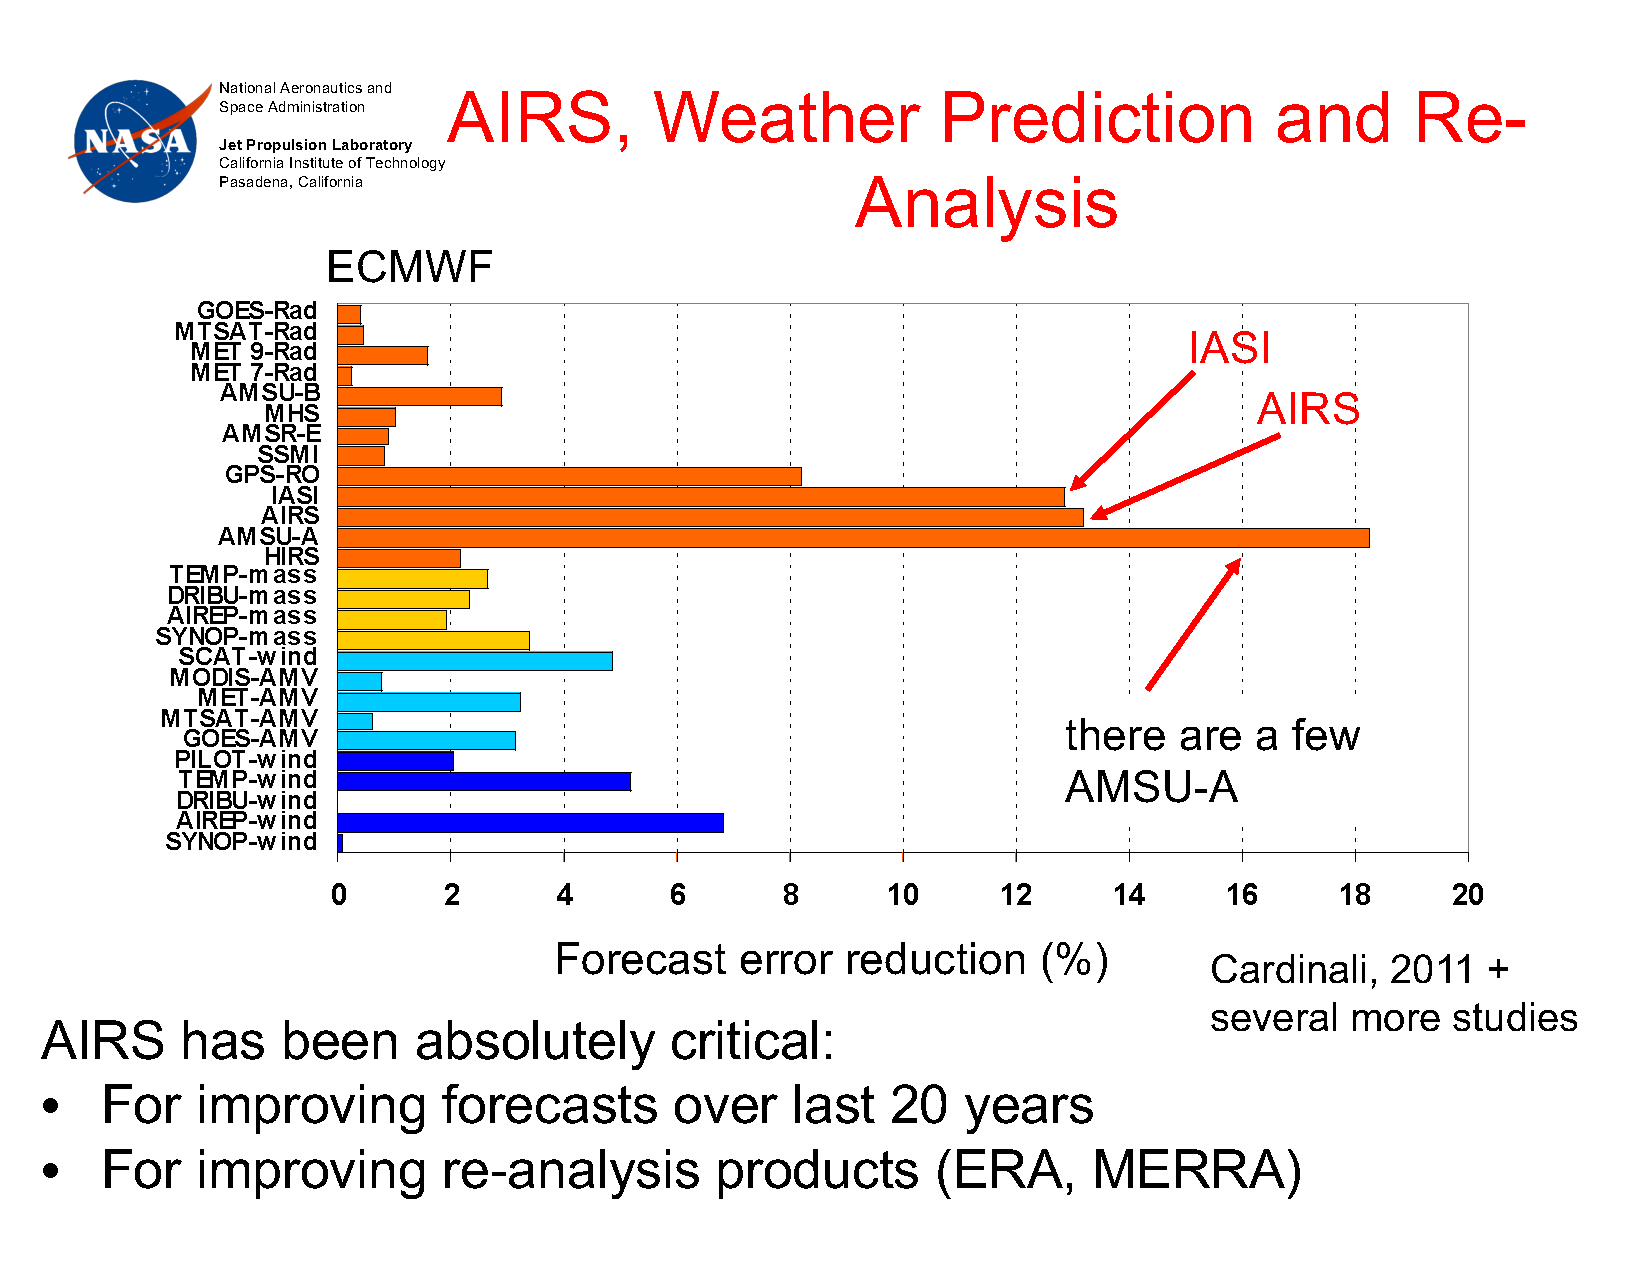
\includepdf[scale=0.80,pages={1}]{Slides_to_Sergio.pdf}
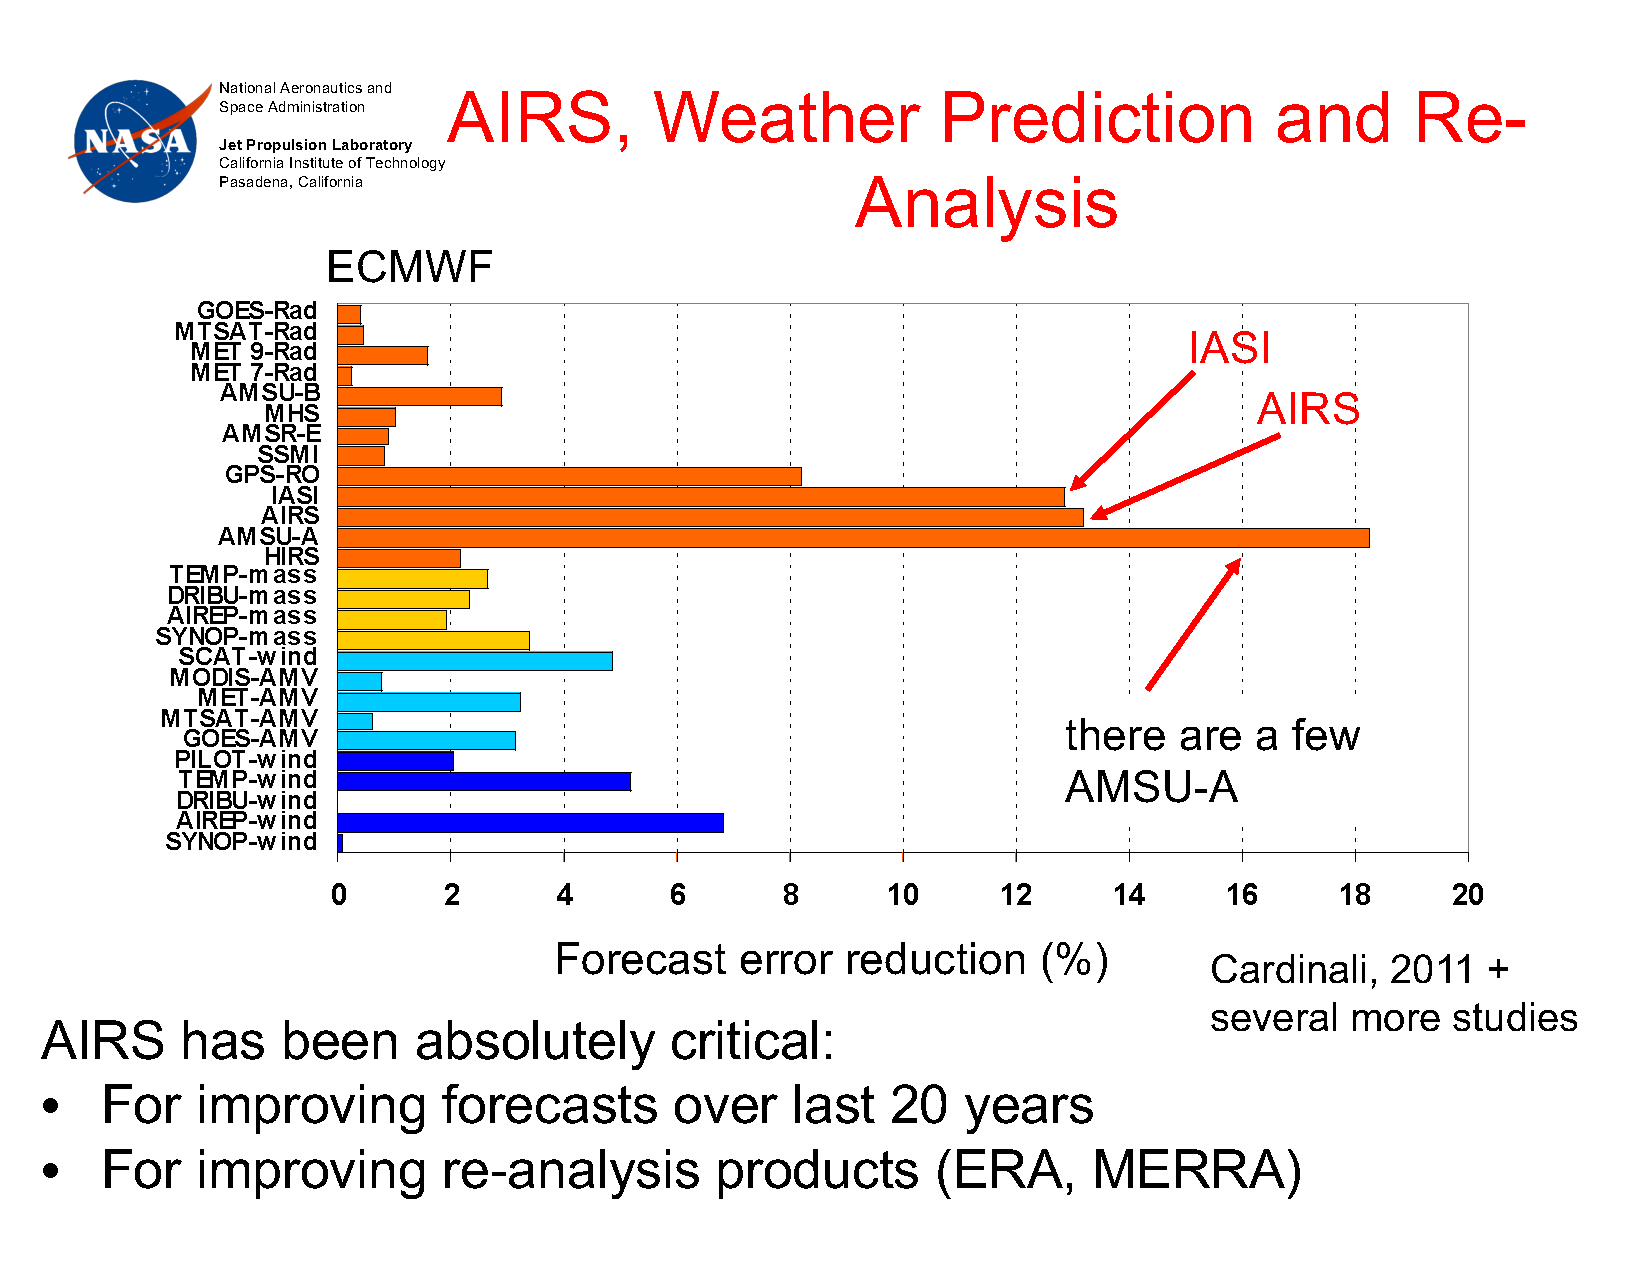
\includegraphics[width=1.01\linewidth,page={1}]{Slides_to_Sergio.pdf}
\end{center}
\end{frame}

%%%%%%%%%%%%%%%%%%%%%%%%%%%%%%%%%%%%%%%%%%%%%%%%%%%%%%%%%%%%%%%%%%%%%%%%
\begin{frame}{L2 Retrievals : AIRS v7 }
\vspace{-0.35in}
\begin{center}
\includegraphics[width=1.01\linewidth,page={7}]{Slides_to_Sergio.pdf}
\end{center}
\end{frame}

\begin{frame}{L2 Retrievals : CLIMCAPS}
\vspace{-0.35in}
\begin{center}
\includegraphics[width=1.01\linewidth,page={8}]{Slides_to_Sergio.pdf}
\end{center}
\end{frame}

%%%%%%%%%%%%%%%%%%%%%%%%%
\begin{frame}{Monitoring Severe Weather}
\vspace{-0.35in}
\begin{center}
\includegraphics[width=1.01\linewidth,page={4}]{Slides_to_Sergio.pdf}
\end{center}
\end{frame}

\begin{frame}{Changes to Severe Weather Storms}
\vspace{-0.35in}
\begin{center}
\includegraphics[width=1.01\linewidth,page={6}]{Slides_to_Sergio.pdf}
\end{center}
\end{frame}

%%%%%%%%%%%%%%%%%%%%%%%%%
\begin{frame}{Helping Understand Science}
\vspace{-0.35in}
\begin{center}
\includegraphics[width=1.01\linewidth,page={2}]{Slides_to_Sergio.pdf}
\end{center}
\end{frame}

\begin{frame}{Helping Understand Science}
\vspace{-0.35in}
\begin{center}
\includegraphics[width=1.01\linewidth,page={3}]{Slides_to_Sergio.pdf}
\end{center}
\end{frame}

\begin{frame}{Helping Understand Science}
\vspace{-0.35in}
\begin{center}
\includegraphics[width=1.01\linewidth,page={9}]{Slides_to_Sergio.pdf}
\end{center}
\end{frame}

%%%%%%%%%%%%%%%%%%%%%%%%%%%%%%%%%%%%%%%%%%%%%%%%%%%%%%%%%%%%%%%%%%%%%%%%
\begin{frame}{Climate Studies and The Future}
\begin{itemize}
  \item AIRS record : 20 years (started 2002/09, still working well)  
  \item Aqua platform running out of power by 2026 (flight maneuvers + come down safely), slowly de-orbit from A-Train
        but still provide data at different time than 1.30 am/pm
  \item NASA may turn mission off in couple years (budget pressure)
  \item CrIS (NOAA) already in orbit for weather purposes \textcolor{red}{CHIRP product for continuity}
\end{itemize}
\end{frame}

\begin{frame}{Overall Approach}
\begin{itemize}
\item Driven by Level 2 + Time \(\neq\) Climate
\item Full sampling not required for climate
\item Manipulate data in radiance space "as long as possible" before retrievals
\item Reduce sensitivity to calibration and RTA bias (radiance anomalies)
\item Optimal estimation retrievals regularized more by smoothing than a-priori
\item Develop analysis approaches that encourage more researchers to use radiances, rather than complicated Level 2 products for climate research, with quick turnaround.
\end{itemize}
%Working to provide CHIRP data on GES DISC AWS Cloud storage in format that allows high-speed I/O for end-user processing of radiances.
\end{frame}

\begin{frame}{AIRS Stability Validation (Clear Ocean Scenes Time Series)}
\vspace{-0.1in}
\begin{center}
%\includegraphics[width=0.65\linewidth]{../../CONFERENCES/SunClimate2022/Strow_JPL_Apr2022/jpl_min//yung/Figs/Pdf/fig10.pdf}
\includegraphics[width=0.65\linewidth]{SunClimate2022/fig10.pdf}
\end{center}

\vspace{-0.05in}
\footnotesize
\begin{itemize}
\item \cd trend (using 400 "good" channels) suggests stability:  -0.023 \textpm{} 0.009 K/decade.  Picks up ENSO related variations in \cd growth at the 0.04K with good S/N
\item \methane and \nitrous trends exhibit small offsets (known events, fixable)
\item (AIRS - GHRSST) SST trends:):  -0.022 \textpm{} 0.012 K/decade
\item This approach provides strong evidence of inherent radiometric stability at the climate level
\end{itemize}
\end{frame}

\begin{frame}{Radiance Sampling}
\begin{itemize}
\item Early testing shows identical surface T trends with 1\%, 3\%, 5\%, and 10\% hottest scenes per 16-day gridded lat/lon cell (3x5 lat/lon).
\item Will this sampling provide accurate profile trends?
\item Careful sampling of cloudier scenes does not preclude retrievals, just more care in cloud parameter a-priori values and parameterization
\begin{itemize}
\item Hyperspectral IR retrievals really need footprint matched cloud parameters from MODIS (like CERES uses).  Univ. Wisconsin has already generated this product for CrIS from VIIRS!
\end{itemize}
\item Subsequent results used 3\% surface T sampling (from 1231 \wn channel)

\vspace{0.1in}
\end{itemize}

Trend retrievals in next few slides take \textasciitilde{}1 hour max, so reprocessing is trivial.\\
  \vspace{0.1in}
Resampling (say for fixed cloud forcing) takes \textasciitilde{}2 days.  
\end{frame}

\begin{frame}{Global IR Radiance Trends and Surface-T Anomalies}
\vspace{-0.35in}

\begin{columns}
\begin{column}{0.55\columnwidth}
\begin{block}{\footnotesize Global Trends: Clear vs All-Sky}
\vspace{-0.1in}
\begin{center}
%\includegraphics[width=\linewidth]{../../CONFERENCES/SunClimate2022/Strow_JPL_Apr2022/jpl_min//Figs1/Pdf/global_trends_hottest3pc_and)allsky.pdf}
\includegraphics[width=\linewidth]{SunClimate2022/global_trends_hottest3pc_and)allsky.pdf}
\end{center}
\end{block}
\end{column}


\begin{column}{0.5\columnwidth}
\begin{block}{\footnotesize Tsurface Global Anomaly}
\vspace{-0.05in}
\begin{center}
%\includegraphics[width=\linewidth]{../../CONFERENCES/SunClimate2022/Strow_JPL_Apr2022/jpl_min//Figs1/Pdf/global_bt1231_anomaly.pdf}
\includegraphics[width=\linewidth]{SunClimate2022/global_bt1231_anomaly.pdf}
\end{center}
\end{block}
\end{column}
\end{columns}

\vspace{-0.1in}
\small
\begin{itemize}
\item "Clear" 3\% hot sampling trends almost same as all-sky
\item Zonally averaged uncertainties (inter-annual variability) \textasciitilde{}0.05K/Decade
\item Good AIRS channels: stability \textasciitilde{}0.02K/Decade
\item Some water band drifts of up to \textasciitilde{}0.04K/Decade (can be fixed)
\item Shortwave known drifts (higher for cold scenes)
\end{itemize}
\end{frame}


\begin{frame}{Follow-On Sensor: SNPP CrIS 8-Year Trends}
\begin{center}
%\includegraphics[width=0.8\linewidth]{../../CONFERENCES/SunClimate2022/Strow_JPL_Apr2022/jpl_min//Figs/Pdf/cris_dbt_clear_all_lats_lwmw_annotated.pdf}
\includegraphics[width=0.8\linewidth]{SunClimate2022/cris_dbt_clear_all_lats_lwmw_annotated.pdf}
\end{center}
\vspace{-0.1in}
\footnotesize Clear ocean scenes \\
\footnotesize Less "hash" due to nature of FTS instrumentation
\end{frame}

\begin{frame}{Spectral Trends}
\begin{center}
\includegraphics[width=0.8\linewidth]{NEWFIGS/model_vs_obs_BTtrends.pdf}
\end{center}
\footnotesize 2002/09-2021/08 trends (ERA5, AIRS V7), 2002/09-2014/08 (CMIP6 ensemble) \newline
\footnotesize UMBC retrieved trends (not shown) agree with AIRS observed trends
\end{frame}

\begin{frame}{Surface Temperature Trend Comparisons}
\vspace{-0.15in}
\begin{center}
%\includegraphics[width=\linewidth]{../../CONFERENCES/SunClimate2022/Strow_JPL_Apr2022/jpl_min//Figs/Png/tsurf_maps_6sources_giss.png}
\includegraphics[width=\linewidth]{SunClimate2022/tsurf_maps_6sources_giss.png}
\end{center}

\vspace{0.1in}
\footnotesize
\begin{center}
\begin{tabular}{lr}
\hline
Data Source & Spatial Correlation\\
 & (w/ UMBC)\\
\hline
CLIMCAPS AIRS & 0.82\\
GISTEMP & 0.74\\
AIRS V7 & 0.70\\
ERA-5 & 0.66\\
MERRA2 & 0.53\\
\hline
\end{tabular}
\end{center}
\end{frame}

\begin{frame}{Zonal T(z) Trends (with CMIP6 to 2014)}
\vspace{-0.15in}
\begin{center}
%\includegraphics[width=\linewidth]{../../CONFERENCES/SunClimate2022/Strow_JPL_Apr2022/jpl_min//Figs/Pdf/zonal_trates_1to1000mbar_cmip6_newcaxis.pdf}
\includegraphics[width=\linewidth]{SunClimate2022/zonal_trates_1to1000mbar_cmip6_newcaxis.pdf}
\end{center}

\footnotesize
IR does have null space near the tropopause.  But trends change sign there as well, as they should.\\
\vspace{0.1in}
UMBC uncertainties \textasciitilde{}0.01K/year (inter-annual variability)
\end{frame}

\begin{frame}{Water Vapor Trends (with CMIP6 to 2014)}
\vspace{-0.15in}
\begin{center}
%\includegraphics[width=\linewidth]{../../CONFERENCES/SunClimate2022/Strow_JPL_Apr2022/jpl_min//Figs/Pdf/zonal_wvrates_50to1000mbar_cmip6.pdf}
\includegraphics[width=\linewidth]{SunClimate2022/zonal_wvrates_50to1000mbar_cmip6.pdf}
\end{center}

\small
\begin{itemize}
\item UMBC a-priori of zero influencing upper-trop WV
\item Quick test using MLS trends as a-priori for UMBC upper-trop
\end{itemize}
\end{frame}

%\begin{frame}[label={sec:org1e985f2}]{Water Vapor Trends (with AURA-MLS: from 2004+)}
%\vspace{-0.15in}
%\begin{center}
%\includegraphics[width=\linewidth]{../../CONFERENCES/SunClimate2022/Strow_JPL_Apr2022/jpl_min//Figs/Pdf/zonal_wvrates_50to1000mbar_mls_umbc_ap_mls.pdf}
%\end{center}
%\vspace{-0.1in}
%\small
%\begin{itemize}
%\item Quick test using MLS trends as a-priori for UMBC upper-trop
%\item MLS water vapor unimportant for OLR applications
%\item Mean global \(\Delta\) RH < 0.01\%/year
%\end{itemize}
%\end{frame}

\begin{frame}{Climate Feedback Estimation from Trend Retrievals}
\vspace{-0.15in}
\small
\begin{itemize}
\item CMIP period ends 2014 compared to our 2002-2021 time period
\item OLR differences directly from trends, no use of inter-annual variability for kernels
\item UMBC results similar to ERA-5 (not shown).
\item Cannot use MERRA2 surface T due to poor trends.
\end{itemize}

\vspace{-0.25in}
\begin{columns}
\begin{column}{0.5\columnwidth}
\begin{block}{\(\lambda\) WV}
\vspace{-0.1in}
\begin{center}
%\includegraphics[width=\linewidth]{../../CONFERENCES/SunClimate2022/Strow_JPL_Apr2022/jpl_min//Figs/Pdf/wvlamda2.pdf}
\includegraphics[width=\linewidth]{SunClimate2022/wvlamda2.pdf}
\end{center}
\end{block}
\end{column}


\begin{column}{0.5\columnwidth}
\begin{block}{\(\lambda\) Lapse Rate}
\vspace{-0.1in}
\begin{center}
%\includegraphics[width=\linewidth]{../../CONFERENCES/SunClimate2022/Strow_JPL_Apr2022/jpl_min//Figs/Pdf/lapselamda2.pdf}
\includegraphics[width=\linewidth]{SunClimate2022/lapselamda2.pdf}
\end{center}
\end{block}
\end{column}
\end{columns}

\vspace{-0.05in}
Note Positive lapse rate feedback in tropics for 2002-2022.
\end{frame}

\begin{frame}{OLR Clear Sky Trends from AIRS (UMBC version)}
\vspace{-0.1in}

\begin{columns}
\begin{column}{0.5\columnwidth}
\begin{block}{\small Total \(\Delta\) OLR (clear) over 19 Years}
\vspace{-0.1in}
\begin{center}
%\includegraphics[width=\linewidth]{../../CONFERENCES/SunClimate2022/Strow_JPL_Apr2022/jpl_min//Figs/Png/ceres_clear_and_cld_19yrold_vs_umbc.png}
\includegraphics[width=\linewidth]{SunClimate2022/ceres_clear_and_cld_19yrold_vs_umbc.png}
\end{center}
\end{block}
\end{column}

\begin{column}{0.5\columnwidth}
\begin{block}{\small Components from AIRS Trends}
\vspace{-0.1in}
\begin{center}
%\includegraphics[width=\linewidth]{../../CONFERENCES/SunClimate2022/Strow_JPL_Apr2022/jpl_min//Figs/Pdf/umbc_olr_components.pdf}
\includegraphics[width=\linewidth]{SunClimate2022/umbc_olr_components.pdf}
\end{center}
\end{block}
\end{column}
\end{columns}

\vspace{-0.05in}

\begin{itemize}
\item UMBC clear closest to CERES All-Sky (but not perfect)
\item Hints for these differences seen in cloud forcing PDFs (in two slides)
\end{itemize}
\end{frame}

\begin{frame}{Summary and Future}
\begin{itemize}

\item Hyperspectral IR observations are a unique dataset to monitor
  and understand climate change, for weather prediction and
  reanalysis, and to evaluate climate models

\item Hyperspectral IR radiances provide insights into the physics of
  the climate system that are not possible using broadband
  observations

\item We are starting to successfully merge hyperspectral IR radiances
  from different instruments which is critical for climate monitoring
  (GPSRO, MLS, MODIS/VIIRS)

\item We will continue to improve these merged products using more
  sophisticated approaches and including additional observations

\item But we need to keep these hyperspectral IR instruments alive and
  stable for as long as technically possible and continue to produce
  climate-level calibrated radiances

\end{itemize}
\end{frame}

\begin{frame}{L1b radiance Stability}
\vspace{-0.35in}
\begin{center}
\includegraphics[width=1.01\linewidth,page={14}]{Slides_to_Sergio.pdf}
\end{center}
\end{frame}

\begin{frame}{Summary}
\vspace{-0.35in}
\begin{center}
\includegraphics[width=1.01\linewidth,page={17}]{Slides_to_Sergio.pdf}
\end{center}
\end{frame}

\begin{frame}{Future}
\vspace{-0.35in}
\begin{center}
\includegraphics[width=1.01\linewidth,page={18}]{Slides_to_Sergio.pdf}
\end{center}
\end{frame}

\end{document}

%%%%%%%%%%%%%%%%%%%%%%%%%%%%%%%%%%%%%%%%%%%%%%%%%%%%%%%%%%%%%%%%%%%%%%%% THE END %%%%%%%%%%%%%%%%%%%%%%%%%
